\documentclass[11 pt]{article}
\usepackage{fullpage,amsthm,amsfonts,amssymb,epsfig,amsmath,times,amsthm}
\usepackage{algorithm,algpseudocode}



\usepackage{pgf, tikz}
\usetikzlibrary{arrows, automata}


\newtheorem{theorem}{Theorem}
\newtheorem{claim}[theorem]{Claim}




\title{ CMPS 102 --- Quarter  Spring 2017 --  Homework 3}
\author{VLADOI MARIAN}
\date{\today}

\begin{document}
\maketitle

\begin{center}
{\bf I have read and agree to the collaboration policy.Vladoi Marian}\\
{\bf I want to choose homework heavy option.}\\
{\bf Name of students I worked with: Victor Shahbazian and Mitchell Etzel }
\end{center}


\section*{Solution to Problem 3: Dynamic Programming}

\textbf{A)} The algorithm from part A , does not correctly solve this example: \\ \\ 

 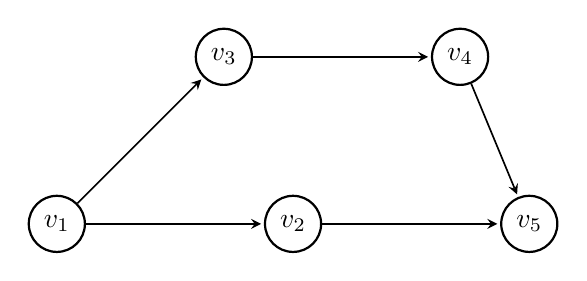
\begin{tikzpicture}[
            > = stealth, % arrow head style
            shorten > = 1pt, % don't touch arrow head to node
            auto,
            node distance = 3cm, % distance between nodes
            semithick % line style
        ]

        \tikzstyle{every state}=[
            draw = black,
            thick,
            fill = white,
            minimum size = 4mm
        ]

        \node[state] (v1) {$v_1$};
        \node[state] (v2) [ right of= v1] {$v_2$};
        \node[state] (v3) [above right of=v1] {$v_3$};
        \node[state] (v4) [right of=v3] {$v_4$};
        \node[state] (v5) [right of=v2] {$v_5$};

        \path[->] (v1) edge node {} (v2);
        \path[->] (v1) edge node {} (v3);
        \path[->] (v2) edge node{} (v5);
        \path[->] (v3) edge node {} (v4);
        \path[->] (v4) edge node {}(v5);
   

      
    \end{tikzpicture}\\ \\ 

The algorithm will chose the path $\{ v_1 , v_2, v_5 \}$ when the correct algorithm would be $\{ v_1 , v_3, v_4, v_5 \}$. \\ \\ 


\textbf{B)}This is my dynamic programming algorithm for finding the longest path
in an ordered graph:\\

The Optimal Substructure :

Lets assume we have an ordered path. $v1$ should be the first node on the path for all $ v_i, i  > 1$. 
Then we have to notice that  there might not be a path from $v_1$ to all nodes $v_i$. Another observation is that: the longest path, in an ordered path, through $v_1$ is one edge longer that the longest path through any node to which $v_1$ is connected.  \\
Notation :   OPT(i) = value of optimal solution to the problem consisting of $v_i$ nodes  i = 1, 2, ..., n.\\

\textbf{   OPT(i) = 0  if i = n }               (we start with the last node in order to use memoisation) \\
 \textbf{  OPT(i) = $- \infty$ }                             ( in case when $v_i $ has no children nodes)\\
\textbf{ OPT(i) = $max_{c \in childredn \ i } \ OPT (1 + OPT(c))$ } (otherwise) ;\\


 The dynamic algorithm for this problem:\\
1. Create an OPT table of size n ( n = number of nodes).\\
2. Create a T stack  (that will store the path nodes, which nodes won the OPT max expression)\\
3. Push $v_n $ to T\\ 
4. Set OPT[n] = 0; \\
3. For i = n - 1 to 1 \\
4. Check the children nodes of i \\
5.  Set OPT[i]= $max_{c \in childredn \ i } \ OPT (1 + OPT(c))$ \\
6. Push the node $v_i$ that wom the max expression to T\\

 The algorithm would fill the OPT table in decreasing order OPT[n], OPT[n-1] ... OPT [1]. We want to make sure that each application of the reccurence will only use precomputed values.
When the for loop terminates OPT[1]  holds the longest path from $v_1$ to $v_n$. \\
The stackT contains the path fron $v_1$ to $v_n$.\\
To reconstruct the path we just pop elements from the stack T . This would have O(n) running time . \\

Proof :
 The value OPT[i] is the longest path  that we can achieve for the subset of nodes $v_1$ to $v_i$. At each step of the for loop iteration we add the node $v_k$  to the longest path from $v_1  \ to \ v_{k-1}$. Assume that at step k, the algorithm choose a solution that is not optimal. Then it would have choosen to add the node $v_k$ to a path that is not the longest path from $v_1  \ to \ v_{k-1}$. We know that this can not happen because we checked which choice result in a longest path  from $v_1  \ to \ v_{k-1}$. in our max OPT expression.  Then  it is garanteed that the solution choosen by the algorithm  is optimal at each node  $v_i$ for $ 0 > i > n$. \\


 Running Time of this algorithm: \\
 n = number of nodes \\
 m = number of edges \\
 Running time  is O( n + m )  \\
 Space  : O(n) . \\
 

\end{document}
